%--------------------------------------------------------------------------------------------------
% OBSERVACAO:
% 
% -> Arquivos que você pode editar:
%    - artigo.tex
%    - artigo_bibliografia.bib
%
% -> Arquivo .TeX codificado em UTF8                                                             
% -> Bibliografia em arquivo .bib (arquivo_bibliografia.bib)                                      
% -> Arquivo de imagens em .jpg, .eps ou .pdf
% -> Para compilar o TeX, execute 'compila_TEX.bat' (terminal do windows)
% 
% versão 1.1 - 19/05/2016
% versão 1.0 - 18/08/2015
%--------------------------------------------------------------------------------------------------
\documentclass{classe_cn}                 % Modelo <nao edite o arquivo classe_cn.cls>
\usepackage[brazil]{babel}                % Acentos
\usepackage[utf8]{inputenc}               % Codificação UTF8 (atenção aqui!)
\usepackage{graphicx}                     % Figura
\usepackage{amssymb}                      % Simbolos matematicos
\usepackage{color}                        % Cores
\usepackage{amsfonts}                     % Fontes
\usepackage{amsmath}                      % Fontes
\usepackage[fixlanguage]{babelbib}        % Acentos
\usepackage[normalem]{ulem}               % OK
\usepackage[retainorgcmds]{IEEEtrantools} % Formulas padrão IEEE
\usepackage{omlmathbf}                    % Simbolos Matematicos
\usepackage{epstopdf}                     % Figuras .eps
\usepackage{setspace}                     % Espaçamento flexível
\usepackage{cmap}                         % Mapear caracteres especiais no PDF
\usepackage{textcomp}                     % Funções e outros símbolos matemáticos
\usepackage{verbatim}                     % Pacotes verbatim
\usepackage{wrapfig}
\usepackage{picins}
\startlocaldefs
\endlocaldefs

%--------------------------------------------------------------------------------------------------
% Inicio do Documento
%--------------------------------------------------------------------------------------------------
\begin{document}
\begin{frontmatter}        % Não alterar
\begin{fmbox}              % Não alterar
\dochead{Gerência da Informação} % Não alterar

%--------------------------------------------------------------------------------------------------
% Titulo do seu Trabalho
%   - pequeno bug (nao funciona cedilha)
%   - editar manualmente o cedilha na classe_cn.cls, linha 1015.
%--------------------------------------------------------------------------------------------------
\title{Software Livre para Empresas}

%------------------------------------------------
% Informações sobre o autor #1
% - Antunes Dantas da Silva
%------------------------------------------------
\author[
  addressref = {aff1},                 % Identifica o autor #1
  email      = {antunes.dantas@ccc.ufcg.edu.br} % email para contato
]
{
  \inits{ADdS}      % Letras iniciais do autor #1
  \fnm{Antunes Dantas}  % Nome do autor #1 (first and middle name)
  \snm{da Silva}   % Ultimo nome do autor #1 (last name)
}
%------------------------------------------------
% Informações sobre o autor #2
% - Gabriel Silva Vinha
%------------------------------------------------
\author[
  addressref = {aff1},                      % Identifica o autor
  email      = {gabriel.vinha@ccc.ufcg.edu.br} % email para contato
]
{
  \inits{GSV}       % Letras iniciais do autor #2
  \fnm{Gabriel Silva}  % Nome do autor #2 (first and middle name)
  \snm{Vinha}    % Ultimo nome do autor #2 (last name)
}
%------------------------------------------------
% Informações sobre o autor #3
% - Italo M. de L. Poroca
%------------------------------------------------
\author[
  addressref = {aff1},                       % Identifica o autor
  email      = {italo.poroca@ccc.ufcg.edu.br} % email para contato
]
{
  \inits{IMdLP}      % Letras iniciais do autor #3
  \fnm{Italo M. de Lima} % Nome do autor #3 (first and middle name)
  \snm{Poroca}    % Ultimo nome do autor #3 (last name)
}
%------------------------------------------------
% Informações sobre o autor #4
% - Valter V. M. de Lucena
%------------------------------------------------
\author[
  addressref = {aff1},                 % Identifica o autor
  email      = {valter.lucena@ccc.ufcg.edu.br} % email para contato
]
{
  \inits{VVMdL}     % Letras iniciais do autor #4
  \fnm{Valter V. M.} % Nome do autor #4 (first and middle name)
  \snm{de Lucena}     % Ultimo nome do autor #4 (last name)
}

%------------------------------------------------
% Endereço dos autores
%------------------------------------------------
\address[id=aff1]{
  \orgname{Universidade Federal de Campina Grande,
           Centro de Engenharia Elétrica e Informática,
           Departamento de Sistemas e Computação},
  \street{Rua Aprígio Veloso, 882, Bairro Universitário},
  \postcode{58429-140},
  \city{Campina Grande},
  \cny{Brasil.}
}

\end{fmbox}

%--------------------------------------------------------------------------------------------------
% Resumo do Trabalho
%--------------------------------------------------------------------------------------------------
\begin{abstractbox}
	
\begin{abstract} 
Escrever no máximo $150$ palavras no resumo do trabalho. Exemplo: The objective of this work is to determine if people are interacting in TV video by detecting whether they are looking at each other or not.We determine both the temporal period of the interaction and also spatially localize the relevant people. We make the following four contributions: (\textit{i}) head detection with implicit coarse pose information (front, profile, back); (\textit{ii}) continuous head pose estimation in unconstrained scenarios (TV video) using Gaussian process regression; (\textit{iii}) propose and evaluate several methods for assessing whether and when pairs of people are looking at each other in a video shot; and (\textit{iv}) introduce new ground truth annotation for this task, extending the TV human interactions dataset. The performance of the methods is evaluated on this dataset, which consists of $300$ video clips extracted from TV shows. Despite the variety and difficulty of this video material, our best method obtains an average precision of $87.6\%$ in a fully automatic manner.
\end{abstract}

%--------------------------------------------------------------------------------------------------
% Palavras-chaves: Entre 3 e 6 palavras chaves
%--------------------------------------------------------------------------------------------------
\begin{keyword}
  \kwd{Escreva}
  \kwd{algumas}
  \kwd{palavras-chaves}
  \kwd{aqui!}
\end{keyword}

\end{abstractbox} % Não alterar
\end{frontmatter} % Não alterar

%--------------------------------------------------------------------------------------------------
% Escreva o seu artigo!
%--------------------------------------------------------------------------------------------------

%------------------------------------------------
% Seção 1
%------------------------------------------------
\section{Introdução}

Escreva introdução e motivação do seu trabalho. Tente convencer o leitor da importância da sua pesquisa. Exemplo: If you read any book on film editing or listen to a director's commentary on a DVD, then what emerges again and again is the importance of eyelines. Standard cinematography practice is to first establish which characters are looking at each other using a medium or wide shot, and then edit subsequent close-up shots so that the eyelines match the point of view of the characters. This is the basis of the well known $180^{o}$ rule in editing.

The objective of this paper is to determine whether eyelines match between characters within a shot—and hence understand which of the characters are interacting~\cite{Pressman:2007}. The importance of the eyeline is illustrated by the three examples of Figure~\ref{tag_figura_01} - one giving rise to arguably the most famous quote from Casablanca, and another being the essence of the humour at that point in an episode of Fawlty Towers. Our target application is this type of edited TV video and films. It is very challenging material as there is a wide range of human actors, camera viewpoints and ever present background clutter. The thirty Brodatz textures u asl sklsksj slk slk dsed are shown in Figure~\ref{tag_figura_01}.

begin
\begin{figure}[h!]
  \begin{center}
    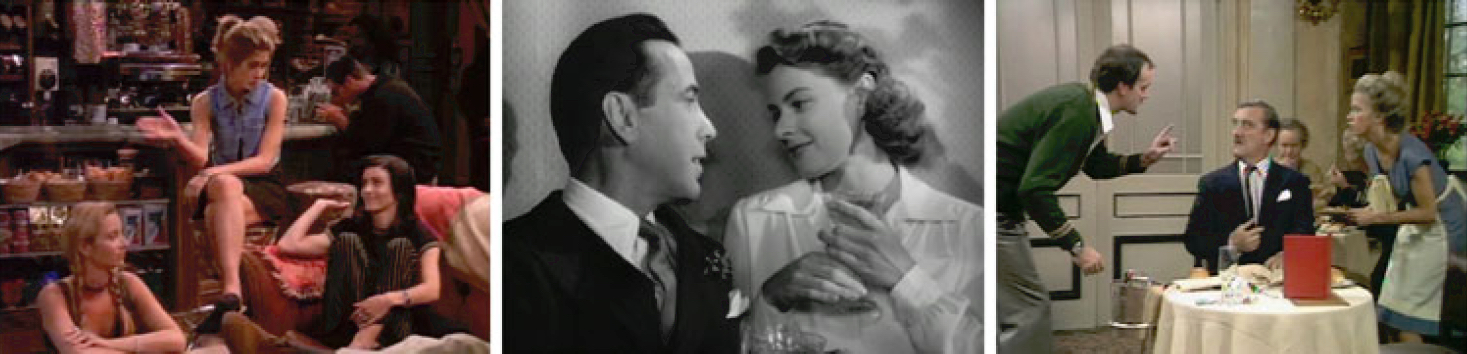
\includegraphics[width=1.0 \textwidth]{figura01.jpg}
    \caption{Exemplo de Figura 01.} 
    \label{tag_figura_01}
  \end{center}
\end{figure}

Gray level co-occurrence matrix (GLCM)~\cite{Ferris:2003} describes the relative frequencies with which two pixels separated by a distance $d$ under a specified angle occur on the image. Then, the GLCM matrices are pre-processed in order to obtain input data for the clustering or classification modules. In the Clustering module the SOM neural network organises and extracts prototypes from the processed matrices, which ends the learning stage. The classification module receives a pre-processed query image and compares it with the prototypes (representations of clusters) obtained in the clustering module. The final result is a list of images belonging to a few number of clusters considered to be the nearest to the user's query. Figure~\ref{tag_figura_02} shows these building blocks.

\begin{figure}[h!]
  \begin{center}
    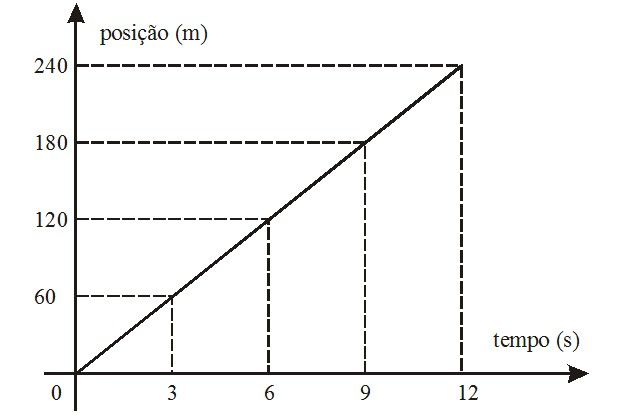
\includegraphics[width=1.0 \textwidth]{figura02.jpg}
    \caption{Exemplo de Figura 02.} 
    \label{tag_figura_02}
  \end{center}
\end{figure}

%------------------------------------------------
% Seção 2
%------------------------------------------------
\section{Motivação}

If we assume that sensitive cells follow a deterministic decay $Z_0(t) = xe^{\lambda_0 t}$ and approximate their extinction time as $T_x \approx \frac{1}{\lambda_0} \log x$, then we can heuristically estimate the expected value as:

\begin{eqnarray}
\label{eqexpmuts}
  E [Z_1(vT_x)] &=& \frac{\mu}{r}\log x \int_0^{1} x^{1-u} du \\
  E [Z_1(vT_x)] &=& \frac{\mu}{r}x^{1-{\lambda_1}/{\lambda_0}v}\log  \\
  1 &=& 10
\end{eqnarray}

\begin{equation}
  E [Z_1(vT_x)] = \frac{\mu}{r}\log x \int_0^{1} x^{1-u} du \\
  E [Z_1(vT_x)] = \frac{\mu}{r}x^{1-{\lambda_1}/{\lambda_0}v}\log 
\end{equation}

Thus we observe that this expected value is finite for all $v>0$ (also see \cite{Rosenfeld:1970}).

%------------------------------------------------
% Sub-seção
%------------------------------------------------
\subsection{Exemplo de Sub-Seção}

In this section we examine the growth rate of the mean of $Z_0$, $Z_1$ and $Z_2$. In addition, we examine a common modeling assumption and note the importance of considering the tails of the extinction time $T_x$ in studies of escape dynamics. We will first consider the expected resistant population at $vT_x$ for some $v>0$, (and temporarily assume $\alpha=0$).

\begin{eqnarray}
E [Z_1(vT_x)]= \mu T_x \int_{0}^{\inf} \lambda_1T_x(v-u)du
\end{eqnarray}

If we assume that sensitive cells follow a deterministic decay $Z_0(t)=xe^{\lambda_0 t}$ and approximate their extinction time as $T_x\approx-\frac{1}{\lambda_0}\log x$, then we can heuristically estimate the expected value as.

%------------------------------------------------
% Exemplo de Tabela
%------------------------------------------------
\section{Software Livre}

Table~\ref{tag_tabela_01} shows the average $ \alpha $ and the standard deviation for the CCR \cite{Rosenfeld:1970} obtained by the \textit{GLCM+SOM} method. We can conclude that for the Brodatz dataset~\cite{Domingues:2010} the processing tool based on mean vectors is the best option~\cite{Rosenfeld:1970, Diday:1989}. Considering this result~\cite{Visible:2013}, the mean vector approach is adopted as processing tool of the \textit{GLCM+SOM} method for the next experiments \cite{Fulano:2009}.

testando 123

% Use a ferramenta para criar tabelas: http://www.tablesgenerator.com/
\begin{table}[h!]
\label{tag_tabela_01}
\caption{Sample table title. This is where the description of the table should go.}
  \begin{tabular}{cccc}
  \hline
       & B1   & B2   & B3   \\ \hline
   A1  & 0.1  & 0.2  & 0.3  \\
   A2  & ...  & ..   & .    \\
   A3  & ..   & .    & .    \\ \hline
  \end{tabular}
\end{table}

\subsection{Software as a Product}

aqui vc faz

\subsection{Software as a Service}

olar

\subsection{Componentes da Produção de Software}

acesso ao software

\section{Licenças de Publicação}

Após o crescimento exponencial da produção de dispositivos eletrônicos e com a popularização dos mesmos,iniciou-se uma grande demanda pela produção de programas lógicos que pudessem tornar os dispositivos físicos mais úteis e aplicáveis para o público em geral. A produção de \textit{software} teve um aumento de mercado e procura, com isso surgiram formas de regulamentação da venda ou distribuição dessas aplicações.

Uma licença de software pode ser caracterizado como uma forma de comportamento relacionada com a redistribuição de \textit{software}, a exemplo dos Estados Unidos, toda distibuição de software está sob a proteção de \textit{copyright} (ou direito de cópia).

O \textit{copyright} é um direito legal que garante ao criador de um trabalho (no caso, desenvolvedores de \textit{software}) direitos exclusivos sobre a sua obra. O código fonte é considerado como propriedade intelectual do autor, podendo ser ele uma empresa, um grupo isolado de desenvolvedores ou um único programador.

As licenças de software garantem ao licenciado (usualmente, o licenciado é o usuário final, ver subseção 1.3) de um \textit{software}, normalmente, uso livre nas fronteiras dos direitos exclusivos do distribuidor. A exceção é a licença de domínio público, onde a cópia, distribuição e modificação são permitidas sobre um código fonte de uma aplicação.
Existem duas licenças maiores que se distinguem em como elas se comportam em relação a duas permissões básicas: o direito de modificar e reusar um \textit{software}. A primeira é a licença proprietária (popularmente conhecida como código fechado), nela, ambos os direitos de modificação e reuso não são licenciados, a outra é a licenças de código \textit{FOSS} (\textit{Free and Open Source Software}) onde ambos os direitos são garantidos para o licenciado.

\begin{table}[h!]
\label{tag_tabela_2}
\caption{Resumo dos direitos garantidos pelas licenças de software}
	\begin{tabular}{ccccc}
	\hline
	Direito de		&	Domínio Público	&	\textit{FOSS}	&	Licença Proprietária \\ \hline
	Cópia	&	Sim	&	Sim	&	Não							\\
	Modificar	&	Sim	&	Sim	&	Não						\\
	Distribuição	&	Sim	&	Sob a mesma licença	&	Não\\ \hline
	\end{tabular}
	\end{table}
	
Alguns exemplos de \textit{software} sob cada uma das licenças são: SQLite e o CERN HTTPd para licenças de domínio público; o kernel do Linux e o \textit{webserver} Apache para licenças de software livre e o Windows e o Mac OSX.
Dentro da licença \textit{FOSS}, várias empresas mantêm definições no tocante as suas licenças. Contudo, a Free Software Foundation segue uma definição mais geral de \textit{software} livre e dispõe de diversas licenças seguindo tal definição. As licenças compatíveis com as orientações da Free Software Foundation são categorizados como produtos sob a licença \textit{copylefted}. Dentro do \textit{copyleft}, temos inúmeros e distintos exemplos de licenças de \textit{software}, um deles é a \textit{General Public License} que garante o direito ilimitado de reprodução, cópia, estudo e modificação. 

Existem também as chamadas licenças permissivas que tem como objetivo estabelecer o mínimo de requerimentos possíveis para a distribuição e uso do \textit{software}. Entre elas estão a licença BSD (\textit{Berkeley Software Distribution}) e a \textit{MIT License}, que obtém o mínimo de restrição no quesito distribuição, porém com livre acesso para uso, estudo, cópia, etc. Assim, licenças permissivas permitem o uso do \textit{software} até mesmo na constituição de um \textit{software} maior com licença proprietária.

\section{Software Livre Para Empresas}


\subsection{Estatísticas De Mercado Para Software Como Um Produto}
oi


\subsection{Software Como Um Serviço}

Serviçoes de software se popularizaram no meio de desenvolvedores como uma ramificação de destinos de produção de software onde há ausência de liberdades. Muito se deve a competitividade e a flexibilidade mudança entre os serviços de um mesmo tipo. O próprio Richard Stallman classificou esse modelo de negócio como intrinsecamente ruim para sua fundação de software livre. 

As licenças \textit{Affero GPL} são licenças derivadas de \textit{FOSS} dedicadas à um exemplo de serviço de software, um provedor de serviços. O provedor de serviços é uma generalização de serviços básicos ou avançados para clientes dedicados à uma rede específica. Existiram duas versões da Affero, a primeira é baseada na segunda versão do \textit{GNU General Public License}, enquanto a segunda versão, que está historicamente ligada com a primeira, e é compatível com a \textit{GNU Affero General Public License}.

Empresas como a RedHat oferecem serviços de \textit{software} sob licenças livres. Um deles é o gerenciador de \textit{cloud services} ManageIQ, que, além de ter seus servços básicos livres, também é de código aberto.

\subsection{core}

\section{Tendências}

olar


%--------------------------------------------------------------------------------------------------
%--------------------------------------------------------------------------------------------------
% Define o arquivo BIB (bibliografia)
%--------------------------------------------------------------------------------------------------
%--------------------------------------------------------------------------------------------------
\bibliographystyle{bmc-mathphys}   % NAO EDITAR!
\bibliography{artigo_bibliografia} % NAO EDITAR! - Bibliography file (usually '*.bib' )

\vspace{1.0cm}
\parpic{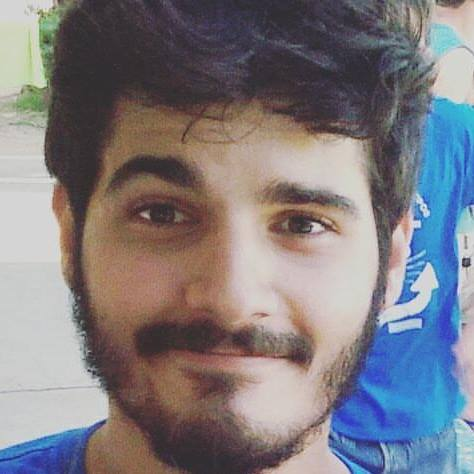
\includegraphics[width=1.5in,clip,keepaspectratio]{gabriel.jpg}}
\noindent {\bf Gabriel Silva Vinha} nasceu no Brasil, no estado de São Paulo e na cidade de São Paulo.Foi selecionado, no ano de 2014, pela embaixada dos Estados Unidos da América como um dos representantes da juventude pelo programa Jovens Embaixadores. Participou do programa de monitoria no Departamento de Sistemas e Computação, na Universidade Federal de Campina Grande. Atualmente, está na graduação em ciência da computação, pela Universidade Federal de Campina Grande. É membro do Laboratório de Sitemas Distribuídos e do \textit{Software Practices Laboratory}. É desenvolvedor part-time em um projeto da parceria entre o Laboratório de Sitemas Distribuídos, \textit{Software Practices Laboratory}, Lenovo Brasil e \textit{RedHat International}. Tem interesse na área de desenvolvimento web, com foco em aplicações e sistemas em nuvem.



%\end{tabular}
%\end{table}

%--------------------------------------------------------------------------------------------------
% FIM DO ARTIGO
%--------------------------------------------------------------------------------------------------
\end{document}
